

\documentclass{sig-alternate-05-2015}

\usepackage{caption} 

\graphicspath{ {images/} }

\def\sharedaffiliation{%
\end{tabular}
\begin{tabular}{c}}

\newcommand{\msg}[1]{\textsc{{#1}}}
\newcommand{\suite}[1]{\texttt{{\footnotesize #1}}}
%mpc: o fim destes comandos é óbvio; se não gostares do aspecto com que ficam as mensagens ou suites podes mudar aqui e fica mudado em todo o artigo


\pagenumbering{arabic} %comment to remove page numbers

\begin{document}

% Copyright
\setcopyright{acmcopyright}
%\setcopyright{acmlicensed}
%\setcopyright{rightsretained}
%\setcopyright{usgov}
%\setcopyright{usgovmixed}
%\setcopyright{cagov}
%\setcopyright{cagovmixed}

% DOI
%\doi{10.475/123_4}

% ISBN
%\isbn{123-4567-24-567/08/06}

%Conference
%\conferenceinfo{ACSAC '16}{June 16--19, 2013, Seattle, WA, USA}

%\acmPrice{\$15.00}

%
% --- Author Metadata here ---
%\conferenceinfo{ACSAC}{'16 El Paso, Texas USA}
%\CopyrightYear{2016} % Allows default copyright year (20XX) to be over-ridden - IF NEED BE.
%\crdata{0-12345-67-8/90/01}  % Allows default copyright data (0-89791-88-6/97/05) to be over-ridden - IF NEED BE.
% --- End of Author Metadata ---

\title{vtTLS: A Vulnerability-Tolerant Communication Protocol}
%vtTLS: A Protocol for Secure Communication Using Diversity and Redundancy

%\subtitle{[Extended Abstract]
%\titlenote{A full version of this paper is available as
%\textit{Author's Guide to Preparing ACM SIG Proceedings Using
%\LaTeX$2_\epsilon$\ and BibTeX} at
%\texttt{www.acm.org/eaddress.htm}}}
%
% You need the command \numberofauthors to handle the 'placement
% and alignment' of the authors beneath the title.
%
% For aesthetic reasons, we recommend 'three authors at a time'
% i.e. three 'name/affiliation blocks' be placed beneath the title.
%
% NOTE: You are NOT restricted in how many 'rows' of
% "name/affiliations" may appear. We just ask that you restrict
% the number of 'columns' to three.
%
% Because of the available 'opening page real-estate'
% we ask you to refrain from putting more than six authors
% (two rows with three columns) beneath the article title.
% More than six makes the first-page appear very cluttered indeed.
%
% Use the \alignauthor commands to handle the names
% and affiliations for an 'aesthetic maximum' of six authors.
% Add names, affiliations, addresses for
% the seventh etc. author(s) as the argument for the
% \additionalauthors command.
% These 'additional authors' will be output/set for you
% without further effort on your part as the last section in
% the body of your article BEFORE References or any Appendices.

\numberofauthors{1} %  in this sample file, there are a *total*
% of EIGHT authors. SIX appear on the 'first-page' (for formatting
% reasons) and the remaining two appear in the \additionalauthors section.
%
\author{
% You can go ahead and credit any number of authors here,
% e.g. one 'row of three' or two rows (consisting of one row of three
% and a second row of one, two or three).
%
% The command \alignauthor (no curly braces needed) should
% precede each author name, affiliation/snail-mail address and
% e-mail address. Additionally, tag each line of
% affiliation/address with \affaddr, and tag the
% e-mail address with \email.
%
% 1st. author
\alignauthor %mpc: ATENÇÃO! A SUBMISSÃO É ANÓNIMA, double-blind review
%Andr\'e Joaquim \ \  \ \ \ Miguel L. Pardal \ \ \ \ \  Miguel Correia\\
%       \affaddr{INESC-ID, Instituto Superior T\'ecnico, Universidade de Lisboa -- Lisbon, Portugal}\\
       %
%       \end{tabular}
%       \begin{tabular}{c}
%       \email{\{andre.joaquim, miguel.pardal, miguel.p.correia\}@tecnico.ulisboa.pt}  
}
% use '\and' if you need 'another row' of author names
% There's nothing stopping you putting the seventh, eighth, etc.
% author on the opening page (as the 'third row') but we ask,
% for aesthetic reasons that you place these 'additional authors'
% in the \additional authors block, viz.
\date{03 May 2016}


\maketitle
\begin{abstract}
We present \textsc{vtTLS}, a vulnerability-tolerant communication protocol based on diversity and redundancy. 
There are often concerns about the strength of some of the encryption mechanisms used in SSL/TLS channels, with some regarded as insecure at some point in time.
\textsc{vtTLS} is our solution to mitigate the problem of secure communication channels being vulnerable to attacks due to unexpected vulnerabilities in encryption mechanisms. It is based on diversity and redundancy of cryptographic mechanisms and certificates to provide a secure communication channel even when one or more mechanisms are vulnerable.
\textsc{vtTLS} relies on a combination of $k$ %mechanisms/
cipher suites.
%amj: são k cipher suites diversas que no total pode originar >k mecanismos
%, whereas $k > 1$ is the diversity factor.
Even if $k - 1$ cipher suites are insecure or vulnerable, \textsc{vtTLS} relies on the remaining cipher suite to maintain the channel secure.
We evaluated the performance of \textsc{vtTLS} by comparing it to an OpenSSL channel.
\end{abstract}

%
% The code below should be generated by the tool at
% http://dl.acm.org/ccs.cfm
% Please copy and paste the code instead of the example below. 
%
\begin{CCSXML}
<ccs2012>
<concept>
<concept_id>10003033.10003039.10003051</concept_id>
<concept_desc>Networks~Application layer protocols</concept_desc>
<concept_significance>500</concept_significance>
</concept>
<concept>
<concept_id>10003033.10003083.10003014</concept_id>
<concept_desc>Networks~Network security</concept_desc>
<concept_significance>300</concept_significance>
</concept>
<concept>
<concept_id>10010520.10010575.10010755</concept_id>
<concept_desc>Computer systems organization~Redundancy</concept_desc>
<concept_significance>500</concept_significance>
</concept>
<concept>
<concept_id>10002978.10003014.10003015</concept_id>
<concept_desc>Security and privacy~Security protocols</concept_desc>
<concept_significance>300</concept_significance>
</concept>
<concept>
<concept_id>10002978.10002979.10002982</concept_id>
<concept_desc>Security and privacy~Symmetric cryptography and hash functions</concept_desc>
<concept_significance>100</concept_significance>
</concept>
</ccs2012>
\end{CCSXML}

\ccsdesc[500]{Networks~Application layer protocols}
\ccsdesc[300]{Networks~Network security}
\ccsdesc[500]{Computer systems organization~Redundancy}
\ccsdesc[300]{Security and privacy~Security protocols}
\ccsdesc[100]{Security and privacy~Symmetric cryptography and hash functions}

%
% End generated code
%

%
%  Use this command to print the description
%
\printccsdesc

\keywords{Protocol; Secure communication channels; Diversity; Redundancy; Vulnerability-Tolerance}

\section{Introduction}
\label{sec-introduction}

\textit{Secure communication protocols} are fundamental building blocks of the current digital economy. \textit{Transport Layer Security} (TLS) alone is responsible for protecting most economic transactions done using the web, with a value so high that it is hard to estimate.

These protocols allow entities to exchange messages or data over a secure channel in the Internet.
A secure communication channel has three properties: \textit{authenticity}, \textit{confidentiality}, and \textit{integrity}. 
Regarding authenticity, in an authenticated channel no one can impersonate the sender.
Regarding confidentiality, in a confidential channel only  the receiver of the message is able to read that message. 
Regarding integrity, the messages can not be modified without the receiver detecting it. 

Several secure communication channel protocols exist no\-wadays,  with different purposes but with the same goal of securing  communication.
%
TLS is a secure communication protocol widely used. Originally called Secure Sockets Layer (SSL), its first  version was SSL 2.0, released in 1995. SSL 3.0 was released in 1996, bringing improvements to its predecessor such as allowing forward secrecy and supporting SHA-1.
Defined in 1999, TLS did not introduce major changes in relation to SSL 3.0.
%, Although, the changes introduced were enough to make TLS 1.0 incompatible with SSL 3.0.
% In order to grant compatibility, a TLS 1.0 connection can be downgraded to SSL 3.0, which brought security issues.
TLS 1.1 and TLS 1.2 are upgrades to TLS 1.0 which brought improvements such as mitigation of cipher block chaining (CBC) attacks and supporting more block cipher modes  to use with AES.
%TLS is divided in two sub-protocols, Handshake and Record, constituted by several mechanisms each. The Handshake protocol is used to establish or re-establish a communication between a server and client. The Record protocol is used to process the sent and received messages.

Other two secure communication protocols are IPsec and SSH.
\textit{Internet Protocol Security} (IPsec) is a network layer protocol that protects the communication at a lower level than SSL/TLS, which operates at application layer \cite{IPsec}. It is an extension of the IP protocol that contains two sub-protocols: AH and ESP.
%
\textit{Secure Shell} (SSH) is an application-layer protocol used for secure remote login and other secure network services over an insecure network \cite{SSH}.

Such a secure communication protocol becomes insecure when a vulnerability is discovered. Vulnerabilities may concern the protocol's specification, the cryptographic mechanisms used, or specific implementations of the protocol. Many vulnerabilities have been discovered in SSL/TLS originating new versions of the protocol with new security features such as deprecating cryptographic mechanisms or enforcing security measures.
Concrete implementations of SSL/ TLS have been also found vulnerable due to implementation bugs, causing  security breaches and affecting devices worldwide.

\textsc{vtTLS} is a protocol that provides \emph{vulnerability-tolerant communication channels}. These channels are characterized by not relying on individual cryptographic mechanisms, so that if one is found vulnerable (or possibly a few of them) the channels remain secure. The idea is to leverage  \textit{diversity}  and \textit{redundancy} of cryptographic mechanisms and keys, i.e., the use respectively of different and more than one set of mechanisms/keys. This use of diversity and redundancy is inspired in previous works on computer immunology \cite{Forrest1997}, diversity in security \cite{Littlewood2004,Garcia:11}, and moving-target defenses \cite{Carvalho2014}.


In the context of \textsc{vtTLS}, diversity and redundancy consist in using two or more different mechanisms with the same objective. For example, SHA-1 and SHA-3 are both hash functions that may be used to generate message digests. If used in combination and  SHA-1 eventually becomes insecure, \textsc{vtTLS} would rely upon SHA-3 to keep the communication secure. %Using diversity and redundancy of cryptographic mechanisms, when a one of those mechanisms is successfully attacked, another mechanism is able to maintain the security and availability of the communication.

\textsc{vtTLS} is configured with a parameter $k$, the \emph{diversity factor} ($k>1$). This parameter indicates the number of different cipher suites and different mechanisms for key exchange, authentication, encryption, and signing. This parameter means also that \textsc{vtTLS} remains secure as long as $k$ vulnerabilities exist. As vulnerabilities and, more importantly, zero-day vulnerabilities that cannot be removed as they are unknown \cite{Bilge:12}, do not appear in large numbers in the same components, we expect $k$ to be usually small, e.g., $k=2$ or $k=3$. 

Although TLS supports strong encryption mechanisms such as AES and RSA, there are factors beyond mathematical complexity that can contribute to vulnerabilities.
Diversifying encryption mechanisms includes diversifying certificates and consequently keys (public, private, shared).
Diversity of certificates is a direct consequence of diversifying encryption mechanisms due to the fact that each certificate is related to an authentication and key exchange mechanism.

The main contribution of this paper is \textsc{vtTLS}, a new protocol for secure communication channels that uses diversity and redundancy to tolerate vulnerabilities in cryptographic mechanisms. It also presents and experimental evaluation of the protocol and shows that it has an acceptable overhead in relation to the TLS implementation in which our prototype is based, OpenSSL v1.0.2g \cite{viega2002network}.

The rest of the document is organized as follows. Section \ref{sec-related-work} presents background and related work. Section \ref{sec-vtTLS} presents the protocol and Section \ref{sec-implementation} its implementation. Section \ref{sec-evaluation} presents the experimental evaluation. Section \ref{sec-conclusions} concludes the paper.


\section{Background and Related Work}
\label{sec-related-work}

%Research was made in order to find previous studies about diversity, how encryption mechanisms can be combined and recent known attacks to secure communication channels, namely SSL/TLS. This section describes research done in these areas.

This section presents related work on diversity (and redundancy) in security, provides background information on TLS, and discusses vulnerabilities in cryptographic mechanisms and protocols.

\subsection{Diversity in Security}

The term \textit{diversity} is used to describe multi-version software in which redundant versions are deliberately created and made different between themselves \cite{Littlewood2004}.
Without diversity, all instances are the same, with the same implementation vulnerabilities. Using diversity it is possible to present the attacker different versions, hopefully with different vulnerabilities. %There is no proper way of knowing the attacks which that particular program is susceptible to.
%
Software diversity targets mostly software implementation and the ability of the attacker to replicate the user's environment. 
Diversity does not change the program's logic, so it is not  helpful if a program is badly designed.
%
According to Littlewood and Strigini, multi-version systems on average are more reliable than those with no versions \cite{Littlewood2004}. They  also state that the key to achieve effective diversity is that the dependence between the different programs needs to be as low as possible. %The best possible effect of diversity would be when the probability of common failure between versions is 0.
%
Therefore, attention is needed when choosing the diverse versions. The trade-off between individual quality and  dependence needs to be assessed and evaluated, as it impacts the correlation between version failures.

%mpc: no fim do paragrafo acima escreve mais alguma coisa sobre o paper do Littlewood; podes tirar ideias da seccao 3.1 da dissertação do Ricardo Carvalho (5o e 6o parags)

%mpc: depois escreve outro paragrafo sobre moving target defenses, com base no que tens no doc de projecto (inicio de 3.2.1.1); idem tirar alguma coisa da seccao 3.1 da dissertação do Ricardo Carvalho, 1o parag, sobre o trab da Forrest

Recently there has been some discussion on the need for moving-target defenses. Such defenses dynamically alter properties of programs and systems in order to overcome vulnerabilities that eventually appear in static defense mechanisms \cite{Evans2011}.
There are two types of moving-target defenses: reactive and proactive \cite{Carvalho2014}. Proactive defenses are generally slower than reactive defenses as they prevent attacks by increasing the system complexity periodically. Reactive defenses are faster as they are activated when they receive a trigger from the system when an attack is detected. This may cause a problem where an attack is performed but  not detected. In this case, reactive defenses are worthless, but  proactive defenses may prevent that attack from being successful.
The best approach would be to implement both \cite{Sousa:10}.
Nevertheless, these defenses are  as good as their ability to make an unpredictable change to the system.

Forrest \emph{et al.}~studied analogies between immunology and computer systems \cite{Forrest1997}.
%and proposed the creation of multiple distributed detectors to attempt detecting malicious code \cite{Forrest1997}. This kind of detectors are classified as reactive defenses, as they are structured to scan for abnormal behaviour. The same authors also
They claimed that introducing diversity in a deliberate fashion into computer systems can make them more robust to replicated attacks \cite{Forrest:1997:BDC:822075.822408}.

%mpc: depois 1 parag sobre N-version programming, com base no que tens em 3.2.2; cita este paper: \cite{Avizienis77n-version}; podes tirar da seccao 3.1 da dissertação do Ricardo Carvalho, 3o paragrafo 

Earlier Avi\v{z}ienis and Chen introduced N-version programming (NVP) \cite{Avizienis77n-version}. NVP is defined as the independent generation of N $\geq 2$ functionally equivalent programs from the same initial specification called \textit{versions}.
%
The authors state that in order to use redundant programs to achieve fault tolerance 
%and, consequently, reliability, three constraints must be met. The last of those constraints refers to the fact that 
the redundant program must contain independently developed alternatives routines for the same functions.

The N in NVP comes from  N diverse versions of a program developed by N different programming teams, or programmers, that do not interact with each other regarding the programming process.
One of the limitations of NVP is that every version is originated from the same initial specification. There is the need to assure the initial specification's correctness, completeness and unambiguity prior to the versions development.

There is some work on obtaining diversity without explicitly  developing N versions \cite{larsen2014sok}. Garcia \emph{et al.}~show that there is enough diversity among operating systems for several practical purpose \cite{Garcia:11}. Homescu \emph{et al.}~use profile-guided optimization for automated software diversity generation \cite{homescu2013profile}. TRR dynamically and randomly relocates program's parts to provide different versions \cite{xu2003transparent}. Proactive obfuscation aims to generate replicas with different vulnerabilities \cite{Roeder:10}



\subsection{SSL/TLS Protocol}

%A secure communication channel is a channel used by two entities to communicate with each other. A secure communication channel ensures confidentiality, authenticity, and integrity. %Confidentiality is defined as keeping information secret. When Alice sends a message to Bob, only Bob can read that message. Confidentiality ensures that no one else will be able to read the message. Authenticity is defined as keeping information authentic. Authenticity ensures that no one tampered the message. Integrity is defined as keeping information honest. Integrity ensures that no one sends a message pretending to be someone else.
%mpc: era repeticao da introducao

This section presents the SSL/TLS, as this is the protocol in which \textsc{vtTLS} is based. We start by presenting its two main sub-protocols: the TLS Handshake Protocol and the TLS Record Protocol.

\subsubsection{TLS Handshake Protocol}

The TLS Handshake Protocol is used to establish or resume a secure session between two communicating parties -- a client and a server.
A session is established in several steps, each one corresponding to a different message:

\begin{enumerate}

\item {The client sends a \msg{ClientHello} message to the server. This message is sent when the client wants to connect to a server.
The \msg{ClientHello} message is composed by the client's TLS version, a structure denominated \textit{Random} (which has a secure random number with 28 bytes and the current date and time), the session identifier, a list of the cryptographic mechanisms supported by the client and a list of compression methods supported by the client, both lists ordered by preference. The client may also request additional functionality from the server.}

%mpc: uma nota sobre Latex: a seguir a \item podes pôr texto à vontade

\item {The server responds with a \msg{ServerHello} message. The message is composed by the server's TLS version, a structure denominated \textit{Random} analogous to \textit{ClientHello}'s structure with the same name, the session identifier, a cryptographic mechanism and a compression method, both of them chosen by the server from the lists received in the \msg{ClientHello} message, and a list of extensions.}

\item {If the key exchange algorithm agreed between client and server requires authentication, the server sends its certificate to the client using a \msg{Certificate} message.}

\item {A \msg{ServerKeyExchange} message is sent to the client after the \msg{Certificate} message if the server's certificate does not contain enough information in order to allow the client to share a premaster secret.}

\item {The server then sends a request for the client's certificate -- \msg{CertificateRequest}. This message is composed by a list of types of certificate the client may send, a list of the server's supported signature algorithms and a list of certificate authorities accepted by the server.}

\item {The server sends a \msg{ServerHelloDone} message to conclude its first sequence of messages.}

\item {After receiving the \msg{ServerHelloDone} message, the client sends its certificate to the server, if requested.
%When the server receives the client's certificate, there are some aspects that may risk the handshake.
If the client does not send its certificate or if its certificate does not meet the server's conditions, the server may choose to continue or to abort the handshake.
}

\item {The client proceeds to send to the server a \msg{ClientKeyExchange} message containing an encrypted premaster secret. The client generates a premaster secret with 48 bytes and encrypts it with the server's certificate public key. At this point, the server and the client use the premaster secret to generate the session keys and the master secret.}

\item {If the client's certificate possesses signing capability, a \msg{CertificateVerify} message is sent to the server. Its purpose is to explicitly verify the client's certificate.}

\item {The client sends a \msg{ChangeCipherSpec} message to the server. This message is used to inform the server that the client is now using the agreed-upon algorithms for encryption and hashing. TLS has a specific protocol to signal transitions in ciphering strategies denominated Change Cipher Spec.
%According to this protocol, a \msg{ChangeCipherSpec} message must be sent by both client and server to notify one another that they are now using the algorithms agreed-upon.
}

\item {The client  sends its last handshake message -- \textit{Finished}. The Finished message verifies the success of the key exchange and the authentication.}

\item {After receiving the \msg{ChangeCipherSpec} message, the server starts using the algorithms established previously and sends a \msg{ChangeCipherSpec} message to the client as well.}

\item {The server puts an end to the handshake protocol by sending a \msg{Finished} message to the client.}

\end{enumerate}

At this point, the session is established. Client and server can now exchange application-layer data through the secure communication channel.


\subsubsection{TLS Record Protocol}

The TLS Record protocol is the sub-protocol which processes the messages to sent and received after the handshake, i.e., in normal operation.

Regarding an outgoing message, the first operation performed by the TLS Record protocol is fragmentation. The message is divided into blocks. %called TLSPlaintext
Each block contains the protocol version, the content type, the fragment of application data and this fragment's length in bytes. The fragment's length must be $2^{14}$ bytes or less.

After fragmenting the message, each block may be optionally compressed, using the compression method defined in the Handshake.
%The compression operation transforms each TLSPlaintext block into a TLSCompressed block. Each TLSCompressed compressed block also contains the protocol version and content type as TLSPlaintext block and contains the compressed form of the fragment and its length. The fragment's length must be $2^{14} \emph{et al.}~ 1024$ bytes or less.
Although there is always an active compression algorithm, the default one is \texttt{CompressionMethod.null}. \texttt{CompressionMethod.null} is an operation that does nothing, i.e., no fields are altered.
%In this case, the TLSCompressed blocks are identical to the TLSPlaintext blocks and no changes are made.

Each potentially compressed block is now transformed into a ciphertext block by encryption and message authentication code (MAC) functions. Each ciphertext block contains the protocol version, content type and the encrypted form of the compressed fragment of application data, with the MAC, and the fragment's length.  The fragment's length must be $2^{14} + 2048$ bytes or less. When using block ciphers, it is also added  padding and its length to the block. The padding is added in order to force the length of the fragment to be a multiple of the block cipher's block length. When using AEAD ciphers, no MAC key is used.
The message is then sent to its destination.

Regarding an incoming message, the process is the inverse. The message is decrypted, verified, optionally decompressed, reassembled and delivered to the application.


%mpc: estas seccoes que descrevem o funcionamento do TLS estão demasiado longas e detalhadas para paper; temos de pensar se vale a pena cortar
%amj: tambem acho que estao um pouco longas, talvez nao valha a pena entrar em tanto detalhe aqui. se calhar vale mais a pena manter mais informacao sobre o Handshake do que propriamente o Record.
%amj: Tentei reduzir um pouco

\subsubsection{TLS Vulnerabilities}
\label{tls-vulnerabilities}

To show the relevance of our work, we discuss some of the vulnerabilities discovered in TLS in the past.
TLS vulnerabilities can be classified in two types: specification vulnerabilities and implementation vulnerabilities. Specification vulnerabilities concern the protocol itself. A specification vulnerability can only be fixed by a new protocol version or an extension. 
%In this section we consider that the deprecation of a cryptographic mechanism is a  design flaw as the protocol should not support an insecure mechanism.
Implementation vulnerabilities exist in the code of some of the  implementations of SSL/TLS, such as OpenSSL.
The Internet Engineering Task Force (IETF) released an RFC in February 2015 summaryzing known TLS attacks and vulnerabilities  \cite{RFC7457}. This section  presents some of the most recent.

The most recent attack against a \emph{specification vulnerability} is Logjam, which was discovered in May 2015 \cite{Adrian2015}. The Logjam  consists in exploiting several Diffie-Hellman key exchange weaknesses.
\textit{Logjam} is a man-in-the-middle attack that downgrades the connection to a weakened Diffie-Hellman mode. TLS supporting Diffie-Hellman with weak parameters is one aspect that makes this attack possible. The other aspect concerns  export cryptography. 
%In the 90's, the USA legislated  restrictions on exporting cryptography. In order to support SSL/TLS in some countries, not allowed to import USA cryptography, SSL/TLS supports weakened Diffie-Hellman modes -- EXPORT modes \cite{Logjam-explained}.
%Previous attacks, such as the one made possible due to the FREAK vulnerability \cite{Beurdouche2015}, have  already used  this weakness of TLS.
%Adrian \textit{et al.} consider Logjam the result of a protocol specification vulnerability due to the fact TLS still allowing the use of Diffie-Hellman with weak parameters \cite{Adrian2015}.
%
%In order to understand the attack itself, the concept of number field sieve algorithm has to be taken into account. A number field sieve algorithm is an efficient algorithm used to factor integers bigger than one hundred digits.
%The authors used a number field sieve algorithm to precompute two weak 512-bit Diffie-Hellman groups used by more than 92\% of the vulnerable servers \cite{Adrian2015}. This measure it taken due to the fact that it is computationally heavy to generate prime numbers with certain characteristics. It is a safe measure for prime numbers with a safe length.
%
This man-in-the-middle attack trades the cipher suites used in the \suite{DHE\_EXPORT} cipher suite, forcing the use of weaker Diffie-Hellman key exchange parameters. As the server supports this valid Diffie-Hellman mode, the handshake proceeds without the server noticing the attack. The server proceeds to compute its premaster secret using weakened Diffie-Hellman parameters. From the client's point-of-view, the server chose a seemingly normal DHE option and proceeds to compute its secret also with weak Diffie-Hellman parameters. At this point, the man-in-the-middle can use the precomputation results to break one of the secrets and establish the connection to the client pretending to be the server. 
%One aspect worth noticing is that this attack will only succeed if the server does not refuse to accept DHE\_EXPORT mode.

%The solution for this vulnerability is simple and has already been implemented. Browsers simply deny the access to servers using weak Diffie-Hellman cipher suites, such as DHE\emph{et al.}~EXPORT, although TLS still allows it.

Regarding \emph{implementation vulnerabilities}, \textit{Heartbleed}, discovered in 2014, is one of the most recent. %Its name is originated from the mechanism where the vulnerability lies, the heartbeat extension. 
Heartbleed was a security vulnerability in OpenSSL 1.0.1 through 1.0.1f, when the heartbeat extension was introduced and enabled by default \cite{heartbeat-extension}. The Heartbleed vulnerability allowed an attacker to perform a buffer over-read, i.e., to read data from the memory of the victim \cite{Carvalho2014-HB}. %A buffer over-read happens when is read more data than allowed. 
%
%Heartbleed can be explained in a very simple manner. OpenSSL trusted the client's input correctness. In a normal heartbeat request, the client sends a message to the server saying: ``If you are alive, send me ``Bob'' which has 3 letters''. The server responds ``Bob''. In a abnormal heartbeat request, the client sends a message to the server saying ``If you are alive, send me ``Bob'' which has 500 letters''. The server responds ``Bob'' followed by 497 bytes taken from the positions of memory following where ``Bob'' was stored.
%
%The server did not check if the real length of the word matched the length the user said the word had.


\subsection{Vulnerabilities in Cryptographic Schemes}

To further motivate the relevance of our work, 
this section presents  vulnerabilities in cryptographic mechanisms, specifically in some of those used by the TLS protocol. %TLS may use a variety of cryptographic mechanisms. Not every mechanism supported by TLS is secure. Several of these mechanism have vulnerabilities which can make the communication insecure, if exploited.
%In this section, we study the vulnerabilities of different cryptographic mechanisms supported by TLS. As our solution intends to use diversity and redundancy to increase security, studying the known vulnerabilities of these mechanisms will help us understand which are the most common vulnerabilities and which mechanisms are secure.

\subsubsection{Public-key Cryptography}

%Proposed by Rivest \emph{et al.} in 1978, RSA is a cryptographic mechanism used to cipher and sign messages or information. RSA's security is based on two problems: factorization of large integers and the RSA problem \cite{Menezes1996}. RSA's strength is inversely proportional to one's available computational power. As the years pass, it is expected that performing the factorization of large integers becomes a possible task.
RSA's security is based on two problems: factorization of large integers and the RSA problem \cite{Menezes1996}.
%amj: adicionei a frase acima para contextualizar
RSA can be considered to be broken when those problems are solved within a practical amount of time.

Kleinjung \emph{et al.}~performed the factorization of RSA-768, a RSA number with 232 digits \cite{Kleinjung2010}. The researchers state they spent almost two years in the whole process, which is clearly a non feasible time.
Factorizing a large integer is  very different  from breaking RSA, which is still secure.
As of 2010, the researchers concluded that RSA-1024 would be factored within five years, i.e., in 2015. As for now, no factorization of RSA-1024 has been publicly announced.

Shor designed a quantum computing algorithm to factorize integers in polynomial time \cite{Shor1995}. However, it requires a quantum computer able to run it, which is still not available.


\subsubsection{Symmetric Encryption}

The Advanced Encryption Standard (AES), originally  Rijndael, 
is the current American standard for symmetric encryption 
%created by Rijmen and Daemen 
\cite{Rijmen2001}. AES can be employed with different key sizes -- 128, 192 or 256 bits. The number of rounds corresponding to each key size is, respectively, 10, 12 and 14.
AES is used by many protocols, including TLS. 
%The growth of its popularity attracted attackers to try to find vulnerabilities in it.

The most successful cryptanalysis of AES was published by Bogdanov \emph{et al.}~in 2011, using a biclique attack, a variant of the MITM attack \cite{Bogdanov2011}. 
%It performed slightly better than brute-force attacks. In order to understand how difficult it is to do the cryptanalysis of AES, 
This attack achieved a complexity of $2^{126.1}$ for the full AES with 128-bit (AES-128). The key is therefore reduced to 126-bit from the original 128-bit, but it would still take many years to successfully attack AES-128.
%Prior to Bogdanov et al., while Rijndael was just a candidate to AES, 
Ferguson \textit{et al.}~presented the first known attacks on the first seven and eight rounds of Rijndael \cite{Ferguson2001}. Although it shows some advance in breaking AES, AES with a key of 128 bits has 10 rounds.

\subsubsection{Hash Functions}

The main applications for hash functions %in modern cryptography 
regard data integrity and message authentication. Sometimes also called message digest or digital fingerprint, the hash is a compact representation of the input string and can be used to uniquely identify that hashed input string \cite{Menezes1996-ch9}.
If a hash function is not preimage resistant or 2nd-preimage resistant, it is therefore vulnerable to preimage attacks. If a hash function is not collision resistant, it is vulnerable to collision attacks.
Some generic attacks to hash function include brute force attacks, birthday attacks and side-channel attacks.

The Secure Hash Algorithm 1 (SHA-1) is a cryptographic hash function which produces a 160-bit message digest. Although there is no public knowledge of collisions for SHA-1, it is no longer recommended \cite{ENISA:14}.
Other attacks have been successful against SHA-1. Stevens \emph{et al.}~presented a freestart collision attack for SHA-1's internal compression function \cite{Stevens15}. Taking into consideration the Damgard-Merkle \cite{Merkle79} construction for hash functions and the input of the compression function, a freestart collision attack is a collision attack where the attacker can choose the initial chaining value, also known as initialisation vector (IV). Although, freestart collision attacks being successful does not imply that SHA-1 is insecure, but it is a step forward in that direction.

In 2005, Wang \emph{et al.}~presented a collision attack on SHA-1 that reduced the number of calculations needed to find collisions from $2^{80}$ to $2^{69}$ \cite{Wang05}. The researchers claim that this was the first collision attack on the full 80-step SHA-1 with complexity inferior to the $2^{80}$ theoretical bound. By the year of 2011, Stevens improved the number of calculations needed to produce a collision from $2^{69}$ to a number between $2^{60.3}$ and $2^{65.3}$ \cite{Stevens11}.

%Nowadays it is still computationally expensive to perform these number of calculations. In the near future,  a collision attack may be affordable for a university research project \cite{Schneier12}.


\section{Vulnerability-Tolerant TLS}
\label{sec-vtTLS}

\textsc{vtTLS} is a protocol for diverse and redundant vulnerabi\-li\-ty-tolerant secure communication channels. It aims at increasing security using diverse and redundant cryptographic mechanisms and certificates. It is based on the TLS protocol. %Although being an independent protocol for secure communication channels, \textsc{vtTLS} is compatible with TLS 1.2.
%mpc: explicar o que é que quer dizer compatível, ou mudar a frase
%amj: neste momento não é compatível, por isso não faz sentido quer a frase existir
The protocol aims to solve the main problem originated by having only one cipher suite negotiated between client and server: when one of the cipher suite's mechanisms becomes insecure, the communication channels using that cipher suite may become vulnerable.
Although most cipher suites' cryptographic mechanisms supported by TLS 1.2 are believed to be secure, Section \ref{sec-related-work} shows clearly that new vulnerabilities may be discovered. 
%there is not any assurance that a governmental agency or a company with high computational power and financial resources is not able to break one of those cryptographic mechanisms in the near future.

Unlike TLS, a \textsc{vtTLS} communication channel does not rely in only one cipher suite. \textsc{vtTLS} negotiates more than one cipher suite between client and server and, consequently, more than one cryptographic mechanism will be used for each \emph{phase}: key exchange, authentication, encryption and MAC.
%
Diversity and redundancy appear firstly in \textsc{vtTLS} in the Handshake protocol, in which client and server negotiate $k$ cipher suites to be used in the communication.
%If the diversity factor is $k=1$ there is no diversity or redundancy, and \textsc{vtTLS} works as regular TLS 1.2, with a single cipher suite.
%amj: actualmente, o vtTLS ainda não está a funcionar com esta feature. como faz tudo 2x (cifrar, etc.), para ser compatível com o TLS tem de existir um mecanismo que o faça perceber que se está a ligar a um servidor TLS e que só pode cifrar 1x e não duas.

The strength of \textsc{vtTLS} resides in the fact that, even when $(k - 1)$ cipher suites become insecure, e.g., because $(k-1)$ of the  cryptographic mechanisms are vulnerable, our protocol remains secure. % The remaining secure, diverse and redundant cipher suite ensures that the communication channel is secured by remaining invulnerable.
The server chooses the best combination of $k$ cipher suites according to the cipher suites server and client have available. However, the choice of the cipher suites might be conditioned by the certificates of both server and client.
Diversity and redundancy will  be introduced in the following communication between client and server. \textsc{vtTLS} uses a subset of the $k$ cipher suites agreed-upon in the Handshake Protocol to encrypt the messages.

%\textsc{vtTLS} negotiates a default of $k = 2$ cipher suites, implying a diversity factor $k = 2$. While performance and management costs must be taken into account, this is the estimate of a reasonable $k$ cipher suites to use in the communication.


%In terms of security, our solution has to tolerate all the attacks given that at least one diverse redundant mechanism of the one attacked should not to be vulnerable that attack. On the contrary, our solution should never be vulnerable to attacks to which TLS is not vulnerable.

\subsection{Protocol Specification}

The \textsc{vtTLS} Handshake Protocol is similar to the TLS Handshake Protocol. The names of the messages are identical in order to provide easier migration and transition from TLS.
%Additionally, all the \textsc{vtTLS} messages' names are analogous to TLS.
%amj: frase duplicada
Using this simplification, the reader familiarized with TLS can more easily understand \textsc{vtTLS}.

The messages that require diversity  are \msg{ClientHello}, \msg{ServerHello}, \msg{ServerKeyExchange}, \msg{k-ServerKey\-Ex\-change}, (Server and Client) \msg{Certificate}, \msg{ClientKeyExchange} and \msg{k-ClientKeyExchange}.

The first message to be sent is  \msg{ClientHello}. Its purpose is to inform the server that the client wants to establish a  secure channel for communication. The content of this message consists in the client's protocol version, a Random structure (analogous to TLS 1.2) containing the current time and a 28-byte pseudo-randomly generated number, the session identifier, a list of the client's cipher suites and a list of the client's compression methods, if compression is to be used.

The server responds with a  \msg{ServerHello} message. This is where the server sends to the client the $k$ cipher suites to be used in the communication. The server also sends its protocol version, a Random structure identical to the one received from the client, the session identifier, and the $k$ cipher suites chosen by the server from the list the client sent. It  also sends the compression method to use, if compression is %to be used in the communication.
enabled.

The server proceeds to send a \msg{(Server) Certificate} message containing its $k$ certificates to the client. The $k$ chosen cipher suites are dependent from the server's certificates. Each certificate is associated with one key exchange mechanism (KEM). Therefore, the $k$ cipher suites must use the key exchange mechanisms supported by the server's certificates.

\textsc{vtTLS} behaves correctly if the server has $c$ certificates, with $0 < c \leq k$ . The cipher suites to be used are chosen considering the available certificates. If $c < k$, the diversity is not fully achieved due to the fact that a number of cipher suites will share the same %certificate
key exchange and authentication mechanisms.

The \msg{ServerKeyExchange} message is the next message to be sent to the client by the server. This message is only sent if one of the $k$ cipher suites includes a key exchange mechanism like ECDHE or DHE that uses ephemeral keys, i.e., that generates new keys for every key exchange. The contents of this message are the server's DH ephemeral parameters. For every other $k - 1$ cipher suites using ECDHE or DHE, the server sends additional \msg{ServerKeyExchange} messages with additional diverse DH ephemeral parameters.
Instead of computing all the ephemeral parameters and sending them all on a single larger message, the server, after computing one parameter, sends it immediately, sending each parameter in a separate message.

\begin{figure}[t]
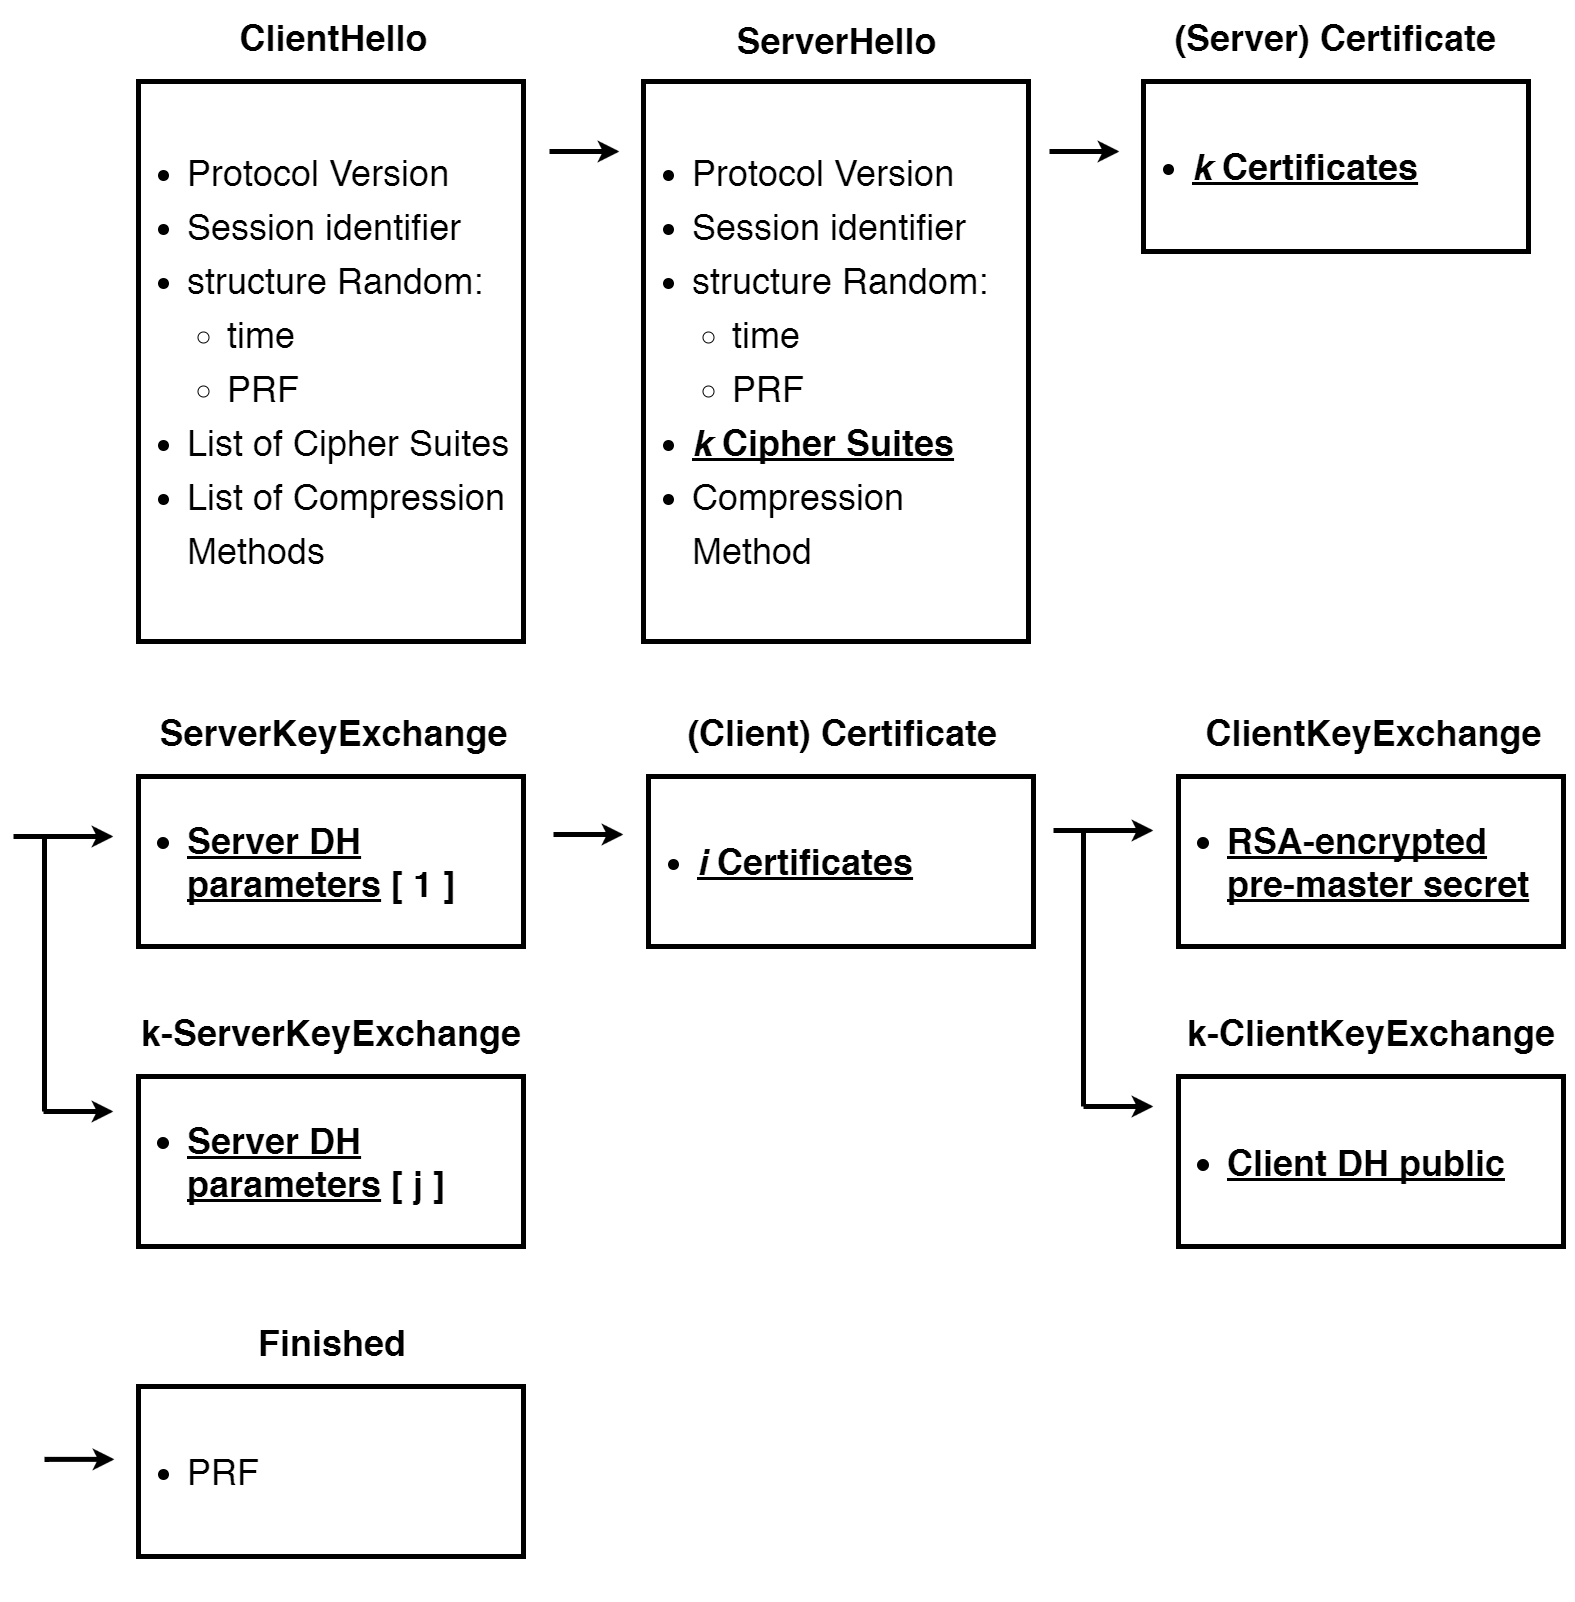
\includegraphics[width=9cm]{vttls-handshake}
\centering
\caption{\textsc{vtTLS} Handshake messages using diversity factor $k$. The places where diversity and redundancy are introduced are marked in bold and underlined.} %places não é muito bonito mas não me lembro de melhor. pode ser "messages" mas tambem nao me soa bem; não pois nem todas são mensagens; items? points? points
\label{fig:vtTLS-example}
\end{figure}

The remaining messages sent by the server to the client at this point of the negotiation, \msg{CertificateRequest} and \msg{ServerHelloDone}, are identical to TLS 1.2 \cite{TLS1.2-5246}.

The client proceeds to send a \msg{(Client) Certificate} message containing its $i$ certificates to the server, analogous to the \msg{(Server) Certificate} message the client received previously from the server.

After sending its certificates, the client sends $k$ \msg{ClientKeyExchange} messages to the server. The content of these messages is based on the $k$ cipher suites chosen. If $m$ of the cipher suites use RSA as KEM, the client sends $m$ messages, each one with a RSA-encrypted pre-master secret to the server ($0 \leq m \leq k$). If $j$ of the cipher suites use ECDHE or DHE, the client sends $j$ messages to the server containing its $j$ Diffie-Hellman public values ($0 \leq j \leq k$). Even if a subset of the $k$ cipher suites share the same KEM, this methodology still applies as we introduce diversity by using different parameters for each cipher suite being used.

The server may need to verify the client's $i$ certificates. If they have signing capabilities, the client digitally signs all the previous handshake messages and sends them to the server for verification.
%mpc: não percebi "If they have signing capabilities". Substitui "they" por aquilo que estás a referir. Mesmo assim não sei se "signing capabilities" se percebe. 
%amj: source - RFC do TLS 1.2: «This message is used to provide explicit verification of a client certificate.  This message is only sent following a client certificate that has signing capability (i.e., all certificates except those containing fixed Diffie-Hellman parameters).»

Client and server now exchange \msg{ChangeCipherSpec} messages, like in the Cipher Spec Protocol of TLS 1.2, in order to state that they are now using the previously negotiated cipher suites for exchanging messages in a secure fashion.

In order to finish the Handshake, the client and server send each other a \msg{Finished} message. This is the first message sent encrypted using the $k$ cipher suites negotiated earlier. Its purpose is to each party receive and validate the data received in this message. If the data is valid, client and server can now exchange messages over the communication channel.

\subsection{Combining Diverse Cipher Suites}
%mpc: agora é tarde mas tinha sido mais interessante pegar na metocologia proposta pelo Ricardo Carvalho e aplicá-la aos mecanismos fornecidos pelo TLS 1.2, em vez de ir dizendo que não estão disponíveis. Possivelmente seria preciso extender algum aspecto dessa metodologia, o que seria ainda mais interessante.
%amj: para a dissertação acho que era interessante fazer isso

Diversity between cryptographic mechanisms can be taken in a soft sense as the use of different mechanisms, or in a hard sense as the use of mechanisms that do not share common vulnerabilities (e.g., because they are based on different mathematical problems). In \textsc{vtTLS} we are interested in using strong diversity in order to claim that no common vulnerabilities will appear in different mechanisms. Measuring the level of diversity is not simple, so we leverage previous research by Carvalho on heuristics for comparing diversity among  cryptographic mechanisms \cite{CarvalhoThesis14}. Moreover, not all cryptographic mechanisms can be used together in the context of TLS 1.2 and other security protocols. 

%mpc: não se percebe o significado das métricas; para a próxima é preciso explicar brevemente cada uma
Diversity can be assessed using different metrics. For hash functions, example metrics are origin, year, digest size, structure, rounds and known weaknesses (collisions, second preimage and preimage).
After comparing several hash functions using the metrics stated above, Carvalho concluded that the best three combinations are the following:
\begin{itemize}
\item {SHA-1 + SHA-3: This combination is not possible in \textsc{vtTLS} as SHA-1 is not recommended and TLS 1.2 does not support SHA-3;}
\item {SHA-1 + Whirlpool: This combination is not possible in \textsc{vtTLS} as SHA-1 is not recommended and TLS 1.2 does not support Whirlpool;} 
\item {SHA-2 + SHA-3: This combination is not possible in \textsc{vtTLS} as TLS 1.2 does not support SHA-3.}
\end{itemize}

All the remaining  combinations suggested in that work cannot also be used because TLS 1.2 does not support SHA-3.
%These results have a direct impact in \textsc{vtTLS} due to the fact that, being \textsc{vtTLS} based on OpenSSL, it also does not support SHA-3 nor Whirlpool. 
All \textsc{vtTLS} cipher suites use either AEAD (MAC-then-Encrypt mode using a SHA-2 variant) or SHA-2 (SHA-256 or SHA-384).
Having a small range of available hash functions limits the maximum diversity factor achievable concerning hash functions.
%SHA-3 is relatively recent, having been selected the winner of the NIST hash function competition on 2012. 
In a near future, it is expected that a new TLS protocol version supports SHA-3 and makes possible the use of diverse hash functions.
Nevertheless, it still possible to achieve diversity by using different variants of SHA-2: SHA-256 and SHA-384.

Regarding public-key functions, the metrics proposed include origin, year, mathematical hard problems, perfect forward secrecy, semantic security and known attacks.
After comparing several public-key encryption mechanisms, using the metrics stated above, Carvalho concluded that the best four combinations are:
\begin{itemize}
\item {DSA + RSA: This combination is possible as TLS 1.2 supports both functions for \textit{authentication}. However, TLS 1.2 specific cipher suites only support DSA with elliptic curves (ECDSA);}
\item {DSA + Rabin-Williams: This combination is not possible as TLS 1.2 does not support Rabin-Williams;}
\item {RSA + ECDH: This combination is possible as TLS 1.2 supports both functions for \textit{key exchange};}
\item {RSA + ECDSA: This combination is possible as TLS 1.2 supports both functions for \textit{authentication}.}
\end{itemize}

Regarding authentication, although DSA + RSA is stated as the most diverse combination, TLS 1.2 preferred cipher suites use ECDSA instead of DSA. Using elliptic curves results in a faster computation and lower power consumption \cite{Gupta02}. With that being said, the preferred combination for authentication is RSA + ECDSA.

Regarding key exchange, the most diverse combination is RSA + ECDH. However, in order to grant perfect forward secrecy, the ECDH with ephemeral keys (ECDHE) has to be employed. Concluding, the preferred combination for key exchange is RSA + ECDHE.
%mpc: logo o critério de fornecer perfect forward secrecy estava omisso na metodologia do Ricardo Carvalho e esta poderia ser afinada
%amj: na proxima iteração, quando fizer entao a metodologia do Ricardo para as cifras do OpenSSL posso referir isso

The study did not present any conclusions regarding sym\-metric-key encryption. Therefore, considering the metrics -- origin, year, and semantic security -- employed for public-key encryption functions, and considering an additional metric -- the mode of operation -- we obtained combinations of diverse symmetric-key encryption functions, all possible:
\begin{itemize}
\item {AES256-GCM + CAMELLIA128-CBC;}
\item {AES256-CBC + CAMELLIA128-GCM;}
\item {AES128-GCM + CAMELLIA256-CBC;}
\item {AES128-CBC + CAMELLIA256-GCM.}
\end{itemize}

Both AES and Camellia are supported by TLS 1.2 and are considered secure. The most diverse combination is AES256-GCM + CAMELLIA128-CBC: the origin of the two algorithms is different, they were first published in different years, they both have semantic security (as they both use initialization vectors) and the mode of operation is also different. One constraint of using this combination is that there is no cipher suite that uses RSA for key exchange, Camellia for encryption and a SHA-2 variant for MAC. Although RFC 6367 \cite{RFC6367} describes the support for Camellia HMAC-based cipher suites, extending TLS 1.2, these cipher suites are not supported by OpenSSL 1.0.2g. Using a cipher suite that uses Camellia, in order to maximize diversity, implies using also SHA-1 for MAC and not using ECDHE for key exchange nor ECDSA for authentication in that cipher suite. Concluding, using Camellia increases diversity in encryption but reduces security in MAC, forcing the use of an insecure algorithm. Nevertheless, diversity in encryption is still an objective to accomplish. We decided that the best option is:
\begin{itemize}
\item {AES256-GCM + AES128: This combination is possible as TLS 1.2 supports both functions.}
\end{itemize}
These functions are, in theory, the same, but employed with a different strength size and mode of operation, they can be considered diverse, although have an inferior degree of diversity comparing to any of the combinations above.

Concluding, the best combination of cipher suites is arguably:
\suite{TLS\_ECDHE\_ECDSA\_WITH\_AES\_256\_GCM\_SHA384} and \suite{TLS\_RSA\_WITH\_AES\_128\_CBC\_SHA256}.
For key exchange,  \textsc{vtTLS} will use Ephemeral ECDH (ECDHE) and RSA; for authentication, it will use Elliptic Curve DSA (ECDSA) and RSA; for encryption, it will use AES-256 with Galois/Counter mode (GCM) and AES-128 with cipher block chaining (CBC) mode; finally, for MAC, it will use SHA-2 variants (SHA-384 and SHA-256).

Using this combination of cipher suites, maximum diversity is achieved using a diversity factor $k = 2$. The least diversified part of the communication is the MAC, due to the fact that TLS 1.2 does not support SHA-3 for now.


\section{Implementation}
\label{sec-implementation}

\textsc{vtTLS}' implementation is a modified version of OpenSSL v1.0.2g.\footnote{\texttt{https://www.openssl.org}} Implementing a secure communication channel from scratch would be a bad option as it might lead to the creation of vulnerabilities; existing software such as OpenSSL has the advantaged of being extensively debugged, although serious vulnerabilities like Heartbleed still appear from time to time.
Furthermore, creating a new secure communication channel, and consequently a new API, would create adoption barriers to programmers otherwise willing to use our protocol. Therefore, we chose to implement \textsc{vtTLS} based on OpenSSL and keeping the same API. Nevertheless, OpenSSL is a huge code base (currently 438,841 lines of code) and modifying it so support diversity was quite a challenge.
%to avoid the maximum amount of vulnerabilities originated from coding errors and to make it easier to migrate from OpenSSL to \textsc{vtTLS}, as the \textsc{vtTLS}' API contains the same functions as the OpenSSL's API plus the \textsc{vtTLS}' specific calls/functions.
%mpc: repetia a mesma coisa; o texto aliás está um bocado repetitivo

\begin{figure*}[tb]
\center\footnotesize
\begin{verbatim}

const char* SSL_get_n_cipher(short n, const SSL* s);
const SSL_CIPHER* SSL_get_current_n_cipher(short n, const SSL* s);
int SSL_CTX_use_n_certificate(short n, SSL_CTX* ctx, X509* x);
int SSL_CTX_use_n_certificate_file(short n, SSL_CTX* ctx, const char* file, int type);
int SSL_CTX_use_n_PrivateKey(short n, SSL_CTX* ctx, EVP_PKEY* pkey);
int SSL_CTX_use_n_PrivateKey_file(short n, SSL_CTX* ctx, const char* file, int type);
int SSL_CTX_check_n_private_key(short n, const SSL_CTX* ctx);
X509* SSL_get_n_peer_certificate(short n, const SSL* s);

\end{verbatim}
\caption{\textsc{vtTLS} API: additional functions in relation to the OpenSSL API.}
\label{fig:vtTLS-api}
\end{figure*}

Although being based on OpenSSL, \textsc{vtTLS} is not compatible with OpenSSL. Due to its diversity and redundancy features, \textsc{vtTLS} can not connect to a OpenSSL server or client. %because, even though it is possible to use \textsc{vtTLS} with just one certificate, even then \textsc{vtTLS} will aim maximizing diversity with the purpose of increasing security.
%
Moreover, the current \textsc{vtTLS} prototype does not support all OpenSSL cipher suites, e.g., PSK and SRP.

\textsc{vtTLS} adds a few functions to the OpenSSL API. These functions are represented in Figure \ref{fig:vtTLS-api}. The meaning of the functions is pretty straightforward. They allow defining additional certificates, keys, cipher functions, etc. The parameter \texttt{n} should be set to the number of the certificate, key, etc.~being added. For example, with $k=2$ the parameter \texttt{n} takes only value $2$ as we have to add just the second of each. For $k=3$ every function has to be called twice, with parameter \texttt{n} set to $2$ and $3$.


In order to establish a \textsc{vtTLS} communication channel, additional functions are required to fulfill the requirements of \textsc{vtTLS}, such as loading two certificates and corresponding private keys. These functions have a similar name of the ones belonging to the OpenSSL API, to reduce the learning curve.
The most relevant functions regarding the setup of the channel are the functions that allow to load the second certificate and private key and allow to check if the second private key corresponds to the second certificate.
%mpc: numa próxima versão era bom listares as funções, ou seja, mostrares a extensão à API; não está muito grande...
%amj: inicialmente era essa a ideia, mas achei que para o artigo ia ficar muito grande. se quiser posso colocar

Regarding the \textit{Handshake Protocol}, we opted for sending $k$ \msg{ServerKeyExchange} and \msg{ClientKeyExchange} messages, instead of sending one single \msg{ServerKeyExchange}, and one single \msg{ClientKeyExchange}, each one with several parameters. This is due to the fact that it is easier to understand and to maintain the code. If $k$ needs to be increased, just send an additional message instead of changing the code related to sending and retrieving \msg{ServerKeyExchange} and \msg{ClientKeyExchange} messages.

The signing and encryption ordering is also  important for \textsc{vtTLS}. Figure \ref{fig:diverse-mac-and-cipher-pt1} shows the ordering for one cipher and one MAC in the OpenSSL implementation.

\begin{figure}[t]
\includegraphics[width=7cm]{diverse_mac_and_cipher_pt1}
\centering
\caption{First four steps regarding the ordering of the encryption and signing of \textsc{vtTLS} using a diversity factor $k = 2$.}
\label{fig:diverse-mac-and-cipher-pt1}
\end{figure}

% This caused some issues regarding the MAC. Applying two MACs in a row, using the same message and the same hash function, which can happen due to TLS' cipher suites using mostly SHA-2 variants, would possibly generate two equal MACs, which is undesirable.

The approach taken was the following, ordered from first to last:
\begin{enumerate}
\item{Apply the first MAC to the plaintext message;}
\item{Encrypt the first message and its MAC with the first encryption function;}
\item{Apply the second MAC to the first ciphertext;}
\item{Encrypt the first ciphertext and its MAC with the second encryption function.}
\end{enumerate}
We opted to maintain the signing prior to the encryption. Using this approach, both message and MACs are encrypted with both ciphers. 
%In this case there is not a chance that both MACs are identical, if the hash function used is secure (SHA-2 is considered secure).
Figure \ref{fig:diverse-mac-and-cipher-pt2} shows the final ordering of \textsc{vtTLS} communication.

\begin{figure}[t]
\includegraphics[width=8cm]{diverse_mac_and_cipher_pt2}
\centering
\caption{Remaining three steps regarding the ordering of the encryption and signing of \textsc{vtTLS} using a diversity factor $k = 2$. Here is represented the second signing and the second encryption, employing diversity and redundancy in the communication.}
\label{fig:diverse-mac-and-cipher-pt2}
\end{figure}


%\subsection{Theoretical Message Size Increase}
%\label{subsec:theoretical-msg-size}

In relation to the \textit{Record Protocol},
signing and encrypting $k$ times has a cost in terms of message size.
Figures \ref{fig:diverse-mac-and-cipher-pt1} and \ref{fig:diverse-mac-and-cipher-pt2} show also the expected
increase of the message size due to the use of a second MAC and a second encryption function (for $k=2$). 
For TLS 1.2 (OpenSSL), the expected size of a message is $first\_len=eivlen+msg\_length+padding+mac\_size$, where $eivlen$ is the size of the initialization vector (IV), $msg\_length$ the original message size, $padding$ the size of the padding in case a block cipher is used, and $mac\_size$ the size of the MAC (Figure \ref{fig:diverse-mac-and-cipher-pt1}). 
For \textsc{vtTLS}, the additional size of the message is $eivlen\_sec+first\_len+padding\_sec+mac\_size\_sec$, where $eivlen\_sec$ is the size of the IV associated with the second cipher and $mac\_size\_sec$ the size of the second MAC.
%mpc: verifica se é isto, sobretudo se a palavra "additional" está certa pois no teu texto não dizias isso; ou seja, a segunda fórmula é para o que se têm a mais em relação ao TLS
%amj: sim, é isto. o "additional MAC" era referente ao second MAC


%old:
%Considering $eivlen$ the size of the initialization vector (IV) associated with the first cipher, $msg\_length$ the original message size and $mac\_size$ the size of the first MAC, Figure \ref{fig:diverse-mac-and-cipher-pt1} shows that the size of the first ciphertext, $first\_len$, using just one encryption and one MAC is equal to $eivlen+msg\_length+mac\_size$. If the encryption function requires a fixed block size, an additional padding of size $padding$ is also added, making the final size $first\_len=eivlen+msg\_length+padding+mac\_size$. This is the expected size of an OpenSSL message.
%For \textsc{vtTLS}, as Figure \ref{fig:diverse-mac-and-cipher-pt2} shows, and as stated before, uses an additional MAC and encryption function. Considering $eivlen\sec$ the size of the IV associated with the second cipher and $mac\_size\_sec$ the size of the second MAC, the size of the second ciphertext is equal to $eivlen\_sec+first\_len+mac\_size\_sec$. Although, similar to the first cipher, if the encryption function requires a fixed block size, a padding of size $padding\_sec$ is also added. Concluding, the final size of the message to be sent is, excluding the header, $eivlen\_sec+first\_len+padding\_sec+mac\_size\_sec$.


In the best case, the number of packets is the same for OpenSSL and \textsc{vtTLS}. In the worst case, one additional packet may be send if the encryption function requires a fixed block size and the maximum size of the packet, after the second MAC and the second encryption, is exceeded by, at least, one byte. In this case, an additional full packet is needed due to the constraint of having fixed block size.

%Concluding, the increase of the message size depends on the length of the second Initialization Vector, the possibly-existent second padding and the length of the second generated MAC.




\section{Experimental Evaluation}
\label{sec-evaluation}

We evaluated \textsc{vtTLS} in terms of two aspects: \textit{performance} and \textit{costs}.
We considered OpenSSL 1.0.2g as the baseline, due to the fact that \textsc{vtTLS} is based on that version of OpenSSL.

Implementing diversity has performance costs and creates overhead in the communication. Every message sent needs to be ciphered and signed $k - 1$ times more than using a TLS implementation, such as OpenSSL, and every message received needs to be deciphered and verified also $k - 1$ times more. In the worst case, users should experience a connection $k$ times slower than using OpenSSL. We considered $k=2$ in all experiments, as this is the value we expect to be used in practice (we expect vulnerabilities to appear rarely, so the ability to tolerate one vulnerability per mechanism sufficient).

In order to perform this tests, we used two virtual machines in the same Intel core i7 computer with 8 GB RAM. The virtual machines run Debian 8 and openSUSE 12 playing the roles of server and client, respectively. All the tests were done in the same controlled environment and same geographic locations in order to maintain the evaluation valid, exact and precise.

\subsection{Performance}

%mpc: depois é preciso fazer esta avaliação com muito mais casos: mais tamanhos, medir a latência da comunicação, o débito que se consegue (numa rede real), etc. etc.
%amj: ok!

In order to evaluate \textsc{vtTLS}' performance, we executed several tests. The main goal was to understand if the overhead of \textsc{vtTLS} is lower, equal, or bigger than $k$ times in relation to OpenSSL.
We configured \textsc{vtTLS} to use the following cipher suites:
\suite{TLS\_RSA\_WITH\_AES\_256\_GCM\_SHA384} and
\suite{TLS\_ECDH\_ECDSA\_WITH\_AES\_256\_GCM\_SHA384}. The suite used with OpenSSL was the second. 


\subsubsection{Handshake}

To evaluate the performance of the handshake, we executed 100 times the Handhake Protocol of both \textsc{vtTLS} and  OpenSSL.
In average, the \textsc{vtTLS}' handshake took 3.909 milliseconds to conclude and the OpenSSL's handshake 2.345 milliseconds. Therefore, the \textsc{vtTLS}'s Handshake takes 66.7\% longer than OpenSSL's Handshake. The \textsc{vtTLS}' Handshake is only 1.67 slower than the OpenSSL's Handshake, which is better than the worst case, 2 times.


\subsection{Data Communication}

After evaluating the Handshake, we performed data communication tests to assess the overhead generated by the diversity and redundancy of mechanisms. As the Handshake, the communication is expected to be at most $k = 2$ times slower than a TLS communication.
For this test, we considered a sample of 100 messages sent and received using \textsc{vtTLS}, and other 100 messages sent and received using OpenSSL. 

\begin{figure}[t]
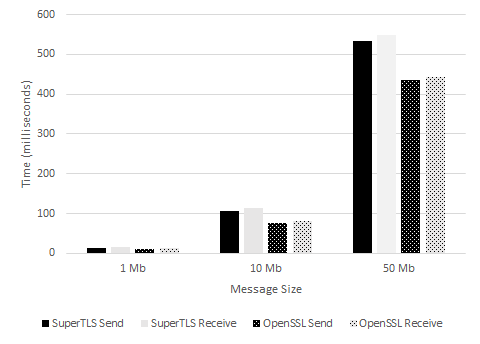
\includegraphics[width=\columnwidth]{eval_time_2_bw}
\centering
\caption{Comparison between the time it takes to send and receive a message using \textsc{vtTLS} and OpenSSL 1.0.2g.}
\label{fig:eval_time_2}
\end{figure}

Figure \ref{fig:eval_time_2} shows the comparison between the time it takes to send and receive a message using \textsc{vtTLS} and
%the time it takes to send, and receive, the same message
OpenSSL/TLS.
The measurements concern the time each channel needs to perform the local operations in order to send the message (including encryption, signing, second encryption and second signing). These values do not include the time taken by the message to reach its destination through the network. The timer is started before the call to \suite{SSL\_write} and stopped after the function returns.
As for the results regarding the reception of messages, the measured time is the time taken to perform the operations necessary to retrieve the message (including second decrypting and second verifying), i.e., the time of execution of \suite{SSL\_read}. 
%amj: já alterei os valores que tinha virgula para ponto, acho que nao me escapou nenhum ok

In average, a message sent through a \textsc{vtTLS} channel takes 22.88\% longer than a message sent with OpenSSL. For example, a 50 MB message takes, in average $534.55$ ms to be sent with \textsc{vtTLS}. Using OpenSSL, the same message takes $435.01$ ms to be sent.
The overhead generated by using diverse encryption and signing mechanisms exists, as expected, but it is much smaller than the worst case.

In Section \ref{sec-implementation}, we  do an analysis of the expected message size increase. In order to validate the premise that the message increase is the same considering the same message size, we measured the increase in the message size comparing once again \textsc{vtTLS} and OpenSSL channels.
A 100 KB plaintext message converts into a ciphertext of $102,771$ bytes  with \textsc{vtTLS}. Using OpenSSL, the same message corresponds to a ciphertext of $102,603$ bytes. Concluding, sending a 100 KB message through \textsc{vtTLS} costs an additional $168$ bytes. Although, as stated before, the number of extra bytes sent is not directly proportional to the message size.

We also evaluated the message size of the ciphertext of a 1 MB plaintext message. A 1 MB plaintext message corresponds to a ciphertext of $1,029,054$ bytes using \textsc{vtTLS}, while using OpenSSL the same message converts into a message of $1,025,856$ bytes. Concluding, sending 1 MB through a \textsc{vtTLS} channel costs an additional $3,198$ bytes than using a OpenSSL channel.

\subsection{Cost}

%\textsc{vtTLS} is a communication channel which objective is to provide a vulnerability-tolerant channel, using diversity and redundancy, to provide security. Nevertheless, %mpc: já tinhas dito isto muitas vezes
Similarly to TLS, \textsc{vtTLS} uses certificates that require some management effort and costs.
A server using OpenSSL/ TLS to protect the communication with clients needs only one certificate. If the administrator decides to use \textsc{vtTLS} instead of TLS, at least $2$ certificates are needed for maximum diversity.
%and at maximum, $k$ certificates.
Although certificates are not  expensive, they represent a cost. %If the cloud or server decides to use \textsc{vtTLS}, it can be used with just one certificate, but diminishing the diversity and, consequently, the potential security increase.
%
Using a diversity factor $k = 2$, the cost associated with certificates duplicates. Nevertheless, we believe that the additional cost of having two certificates instead of one is compensated by the increase in security and vulnerability tolerance provided by \textsc{vtTLS}.
%
Regarding management, there is the need to manage two certificates instead of one. This does not represent a substantial increase in management effort. %If the administrator decides to use \textsc{vtTLS} with a diversity factor $k > 2$, the management costs of maintaining $k$ certificates might represent an significant increase of management costs.



\section{Conclusions}
\label{sec-conclusions}

\textsc{vtTLS} is a diverse and redundant vulnerability-tolerant secure communication protocol designed for communication between clouds. It aims at increasing security using  diverse cipher suites to tolerate vulnerabilities in the encryption mechanisms used in the communication channel. 
%We used a default diversity factor $k = 2$ for \textsc{vtTLS}, and the preferred cipher suite to use with a \textsc{vtTLS} are \suite{TLS\_ECDHE\_ECDSA\_WITH\_AES\_256\_GCM\_SHA384} and \suite{TLS\_RSA\_WITH\_AES\_128\_CBC\_SHA256}. 
In order to evaluate our solution, we compared it to an OpenSSL 1.0.2g communication channel. While expected to be $k = 2$ times slower than an OpenSSL channel, the evaluation showed that using diversity and redundancy of cryptographic mechanisms in \textsc{vtTLS} does not generate such a high overhead. \textsc{vtTLS} takes, in average, 22.88\% longer to send a message than TLS/OpenSSL, but considering the increase in security, this overhead is acceptable.
Overall, considering the additional costs of having an extra certificate, the time increase, and potential management costs,  \textsc{vtTLS} seems to provide an interesting trade-off for a set of critical applications.
%for clouds to communicate,
%amj: "good" não me parece um adjetivo muito... científico
%mpc: pois; resolvi
%using diversity to mitigate existent vulnerabilities.

%\end{document}  % This is where a 'short' article might terminate

%ACKNOWLEDGMENTS are optional
%\section{Acknowledgments}
%This section is optional; it is a location for you
%to acknowledge grants, funding, editing assistance and
%what have you.  In the present case, for example, the
%authors would like to thank Gerald Murray of ACM for
%his help in codifying this \textit{Author's Guide}
%and the \textbf{.cls} and \textbf{.tex} files that it describes.

%\section{Future Work}
%
%\begin{itemize}
%\item{vtTLS is based only on a version of OpenSSL. An interesting feature would be diversifying two different libraries and make them compatible with each other. This would increase diversity in the code and, optionally, programming languages. Also, different teams think differently and this could potentially lead to make vtTLS to tolerate more vulnerabilities regarded with the implementation;}
%\item{Using SHA-3 for hash to increase diversity when it is supported by TLS}
%\item{vtTLS performed rather well comparing with OpenSSL. The only existing approach other than vtTLS is TLS-over-TLS. Future work: Compare vtTLS with TLS-over-TLS.}
%\end{itemize}

%
% The following two commands are all you need in the
% initial runs of your .tex file to
% produce the bibliography for the citations in your paper.
\bibliographystyle{abbrv}
\bibliography{sigproc}  % sigproc.bib is the name of the Bibliography in this case
% You must have a proper ".bib" file
%  and remember to run:
% latex bibtex latex latex
% to resolve all references
%
% ACM needs 'a single self-contained file'!
%
%\section{References}
%Generated by bibtex from your ~.bib file.  Run latex,
%then bibtex, then latex twice (to resolve references)
%to create the ~.bbl file.  Insert that ~.bbl file into
%the .tex source file and comment out
%the command \texttt{{\char'134}thebibliography}.
% This next section command marks the start of
% Appendix B, and does not continue the present hierarchy
%\section{More Help for the Hardy}
%The sig-alternate.cls file itself is chock-full of succinct
%and helpful comments.  If you consider yourself a moderately
%experienced to expert user of \LaTeX, you may find reading
%it useful but please remember not to change it.
%\balancecolumns % GM June 2007
% That's all folks!
\end{document}
